\section{Information-theoretic analysis of the three recorded strokes}\label{app:info}

\emph{Shannon entropy, bits and nats, KL divergence, Bayes' theorem and two-event conditional problems.}

\subsection{Data, variables and labels}

The recording contains \textbf{three topspin strokes} in one trial (379 frames, \SI{60}{\hertz}). Using the same paddle proxy as the Vizard scene (left wrist $+\SI{0.10}{\meter}$ along the forearm), the proxy speed has three clear forward-swing peaks. Each stroke is analysed in a window of $\pm15$ frames ($\pm\SI{0.25}{\second}$, 31 frames) around its peak. Everything below is computed from the recorded kinematics and the geometric criterion of Eq.~\eqref{eq:criterion}, so it is \tagobs{} (kinematics) or \tagsim{} (ball placement and criterion); the observer example in Problem~5 uses assumed rates and is \tagill{}, not participant data.

\begin{table}[ht]
    \centering
    \caption{The three strokes (Vizard axes: $X$ right, $Y$ up, $Z$ forward). The RMS radial spread of the three impact points about their mean is \textbf{0.068 m}, which is $72\,\%$ of the contact threshold $\Rc=\SI{0.095}{\meter}$.}\label{tab:strokes}
    \footnotesize
    \begin{tabularx}{\textwidth}{@{}l c c c c Y@{}}
        \toprule
        \textbf{Stroke} & \textbf{Frame} & $t$ (s) & \textbf{Peak speed (m/s)} & \textbf{Impact point $x,y,z$ (m)} & \textbf{Distance to the other strokes' impact points} \\
        \midrule
        S1              & 101            & 1.683   & 7.72                      & $-0.459,\ 1.192,\ 0.112$          & 0.083 m (S2), 0.121 m (S3)                            \\
        S2 (reference)  & 185            & 3.083   & 7.84                      & $-0.412,\ 1.175,\ 0.178$          & 0.083 m (S1), 0.142 m (S3)                            \\
        S3              & 260            & 4.333   & 7.26                      & $-0.392,\ 1.111,\ 0.052$          & 0.121 m (S1), 0.142 m (S2)                            \\
        \bottomrule
    \end{tabularx}
\end{table}

\textbf{Why this matters for the affordance.} The report's boundary was computed from stroke S2 alone. The stroke-to-stroke spread of the impact point ($\approx\SI{7}{\centi\meter}$) is of the same size as the boundary (\SI{9.5}{\centi\meter}) and larger than the \SI{1.5}{\centi\meter} margin of C2, so the affordance is better described as a \textbf{probability} than as a sharp yes/no. Information theory gives the tools to say this in bits.

\subsection{Entropy, bits and nats}

For a discrete variable with probabilities $p_i$, the Shannon entropy is $H=-\sum_i p_i\log p_i$. With $\log_2$ the unit is the \textbf{bit}; with the natural logarithm it is the \textbf{nat}. They differ only by a constant: $H_{\mathrm{nats}}=H_{\mathrm{bits}}\ln 2$ (1 bit $=0.6931$ nats; 1 nat $=1.4427$ bits). The distribution used is the \emph{occupancy} of proxy speed: the fraction of frames spent in each \SI{1}{\meter\per\second} bin (8 bins, maximum entropy $\log_2 8=3$ bits). It describes how widely the stroke spreads over speeds; frames are autocorrelated, so it is not a sample of independent trials.

\begin{table}[ht]
    \centering
    \caption{Entropy of the proxy-speed occupancy \tagobs. The plug-in estimate is biased low for 31 frames in 8 bins by about $(K-1)/(2N)=0.11$ nats (0.16 bits, Miller--Madow); the three strokes are affected equally.}\label{tab:entropy}
    \footnotesize
    \begin{tabularx}{\textwidth}{@{}l c c c c Y@{}}
        \toprule
        \textbf{Distribution} & \textbf{Frames} & $H$ (bits) & $H$ (nats) & $H/3$ bits & \textbf{Reading}                                                                                     \\
        \midrule
        Whole trial           & 379             & 2.443      & 1.693      & 81\,\%     & Mostly slow frames (146 frames below \SI{1}{\meter\per\second}), so the distribution is concentrated \\
        Stroke 1 window       & 31              & 2.877      & 1.994      & 96\,\%     & Nearly uniform over speeds: acceleration and deceleration                                            \\
        Stroke 2 window       & 31              & 2.868      & 1.988      & 96\,\%     & Same as S1                                                                                           \\
        Stroke 3 window       & 31              & 2.922      & 2.025      & 97\,\%     & Slightly more spread (lower peak, \SI{7.26}{\meter\per\second})                                      \\
        \bottomrule
    \end{tabularx}
\end{table}

\begin{figure}[ht]
    \centering
    \begin{subfigure}{0.48\textwidth}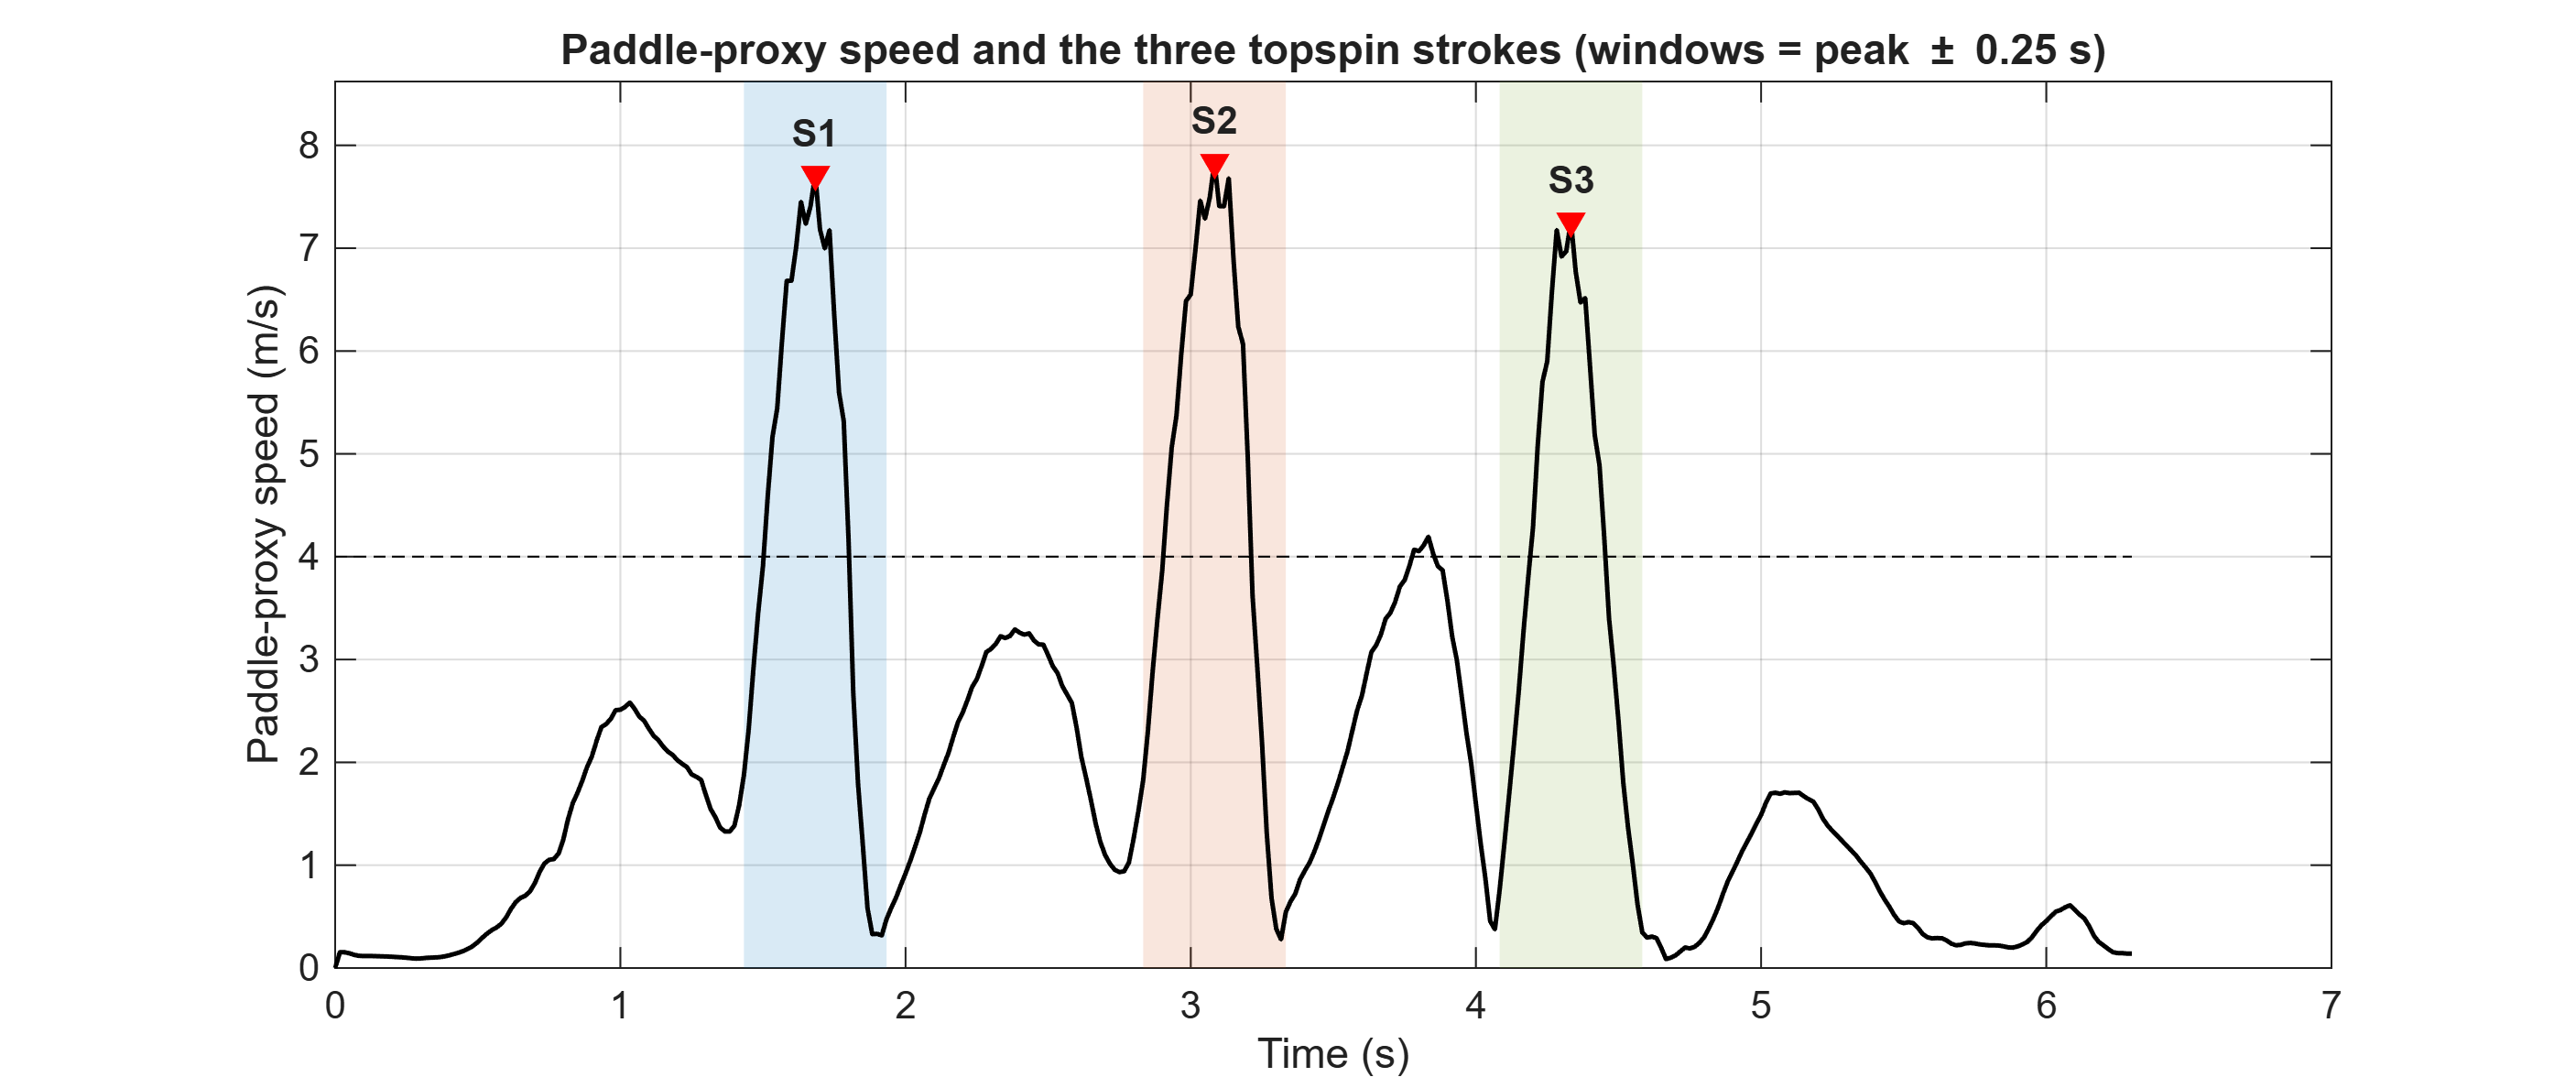
\includegraphics[width=\linewidth]{Fig1_speed_timeseries.png}\caption{Proxy speed, three stroke windows}\end{subfigure}\hfill
    \begin{subfigure}{0.48\textwidth}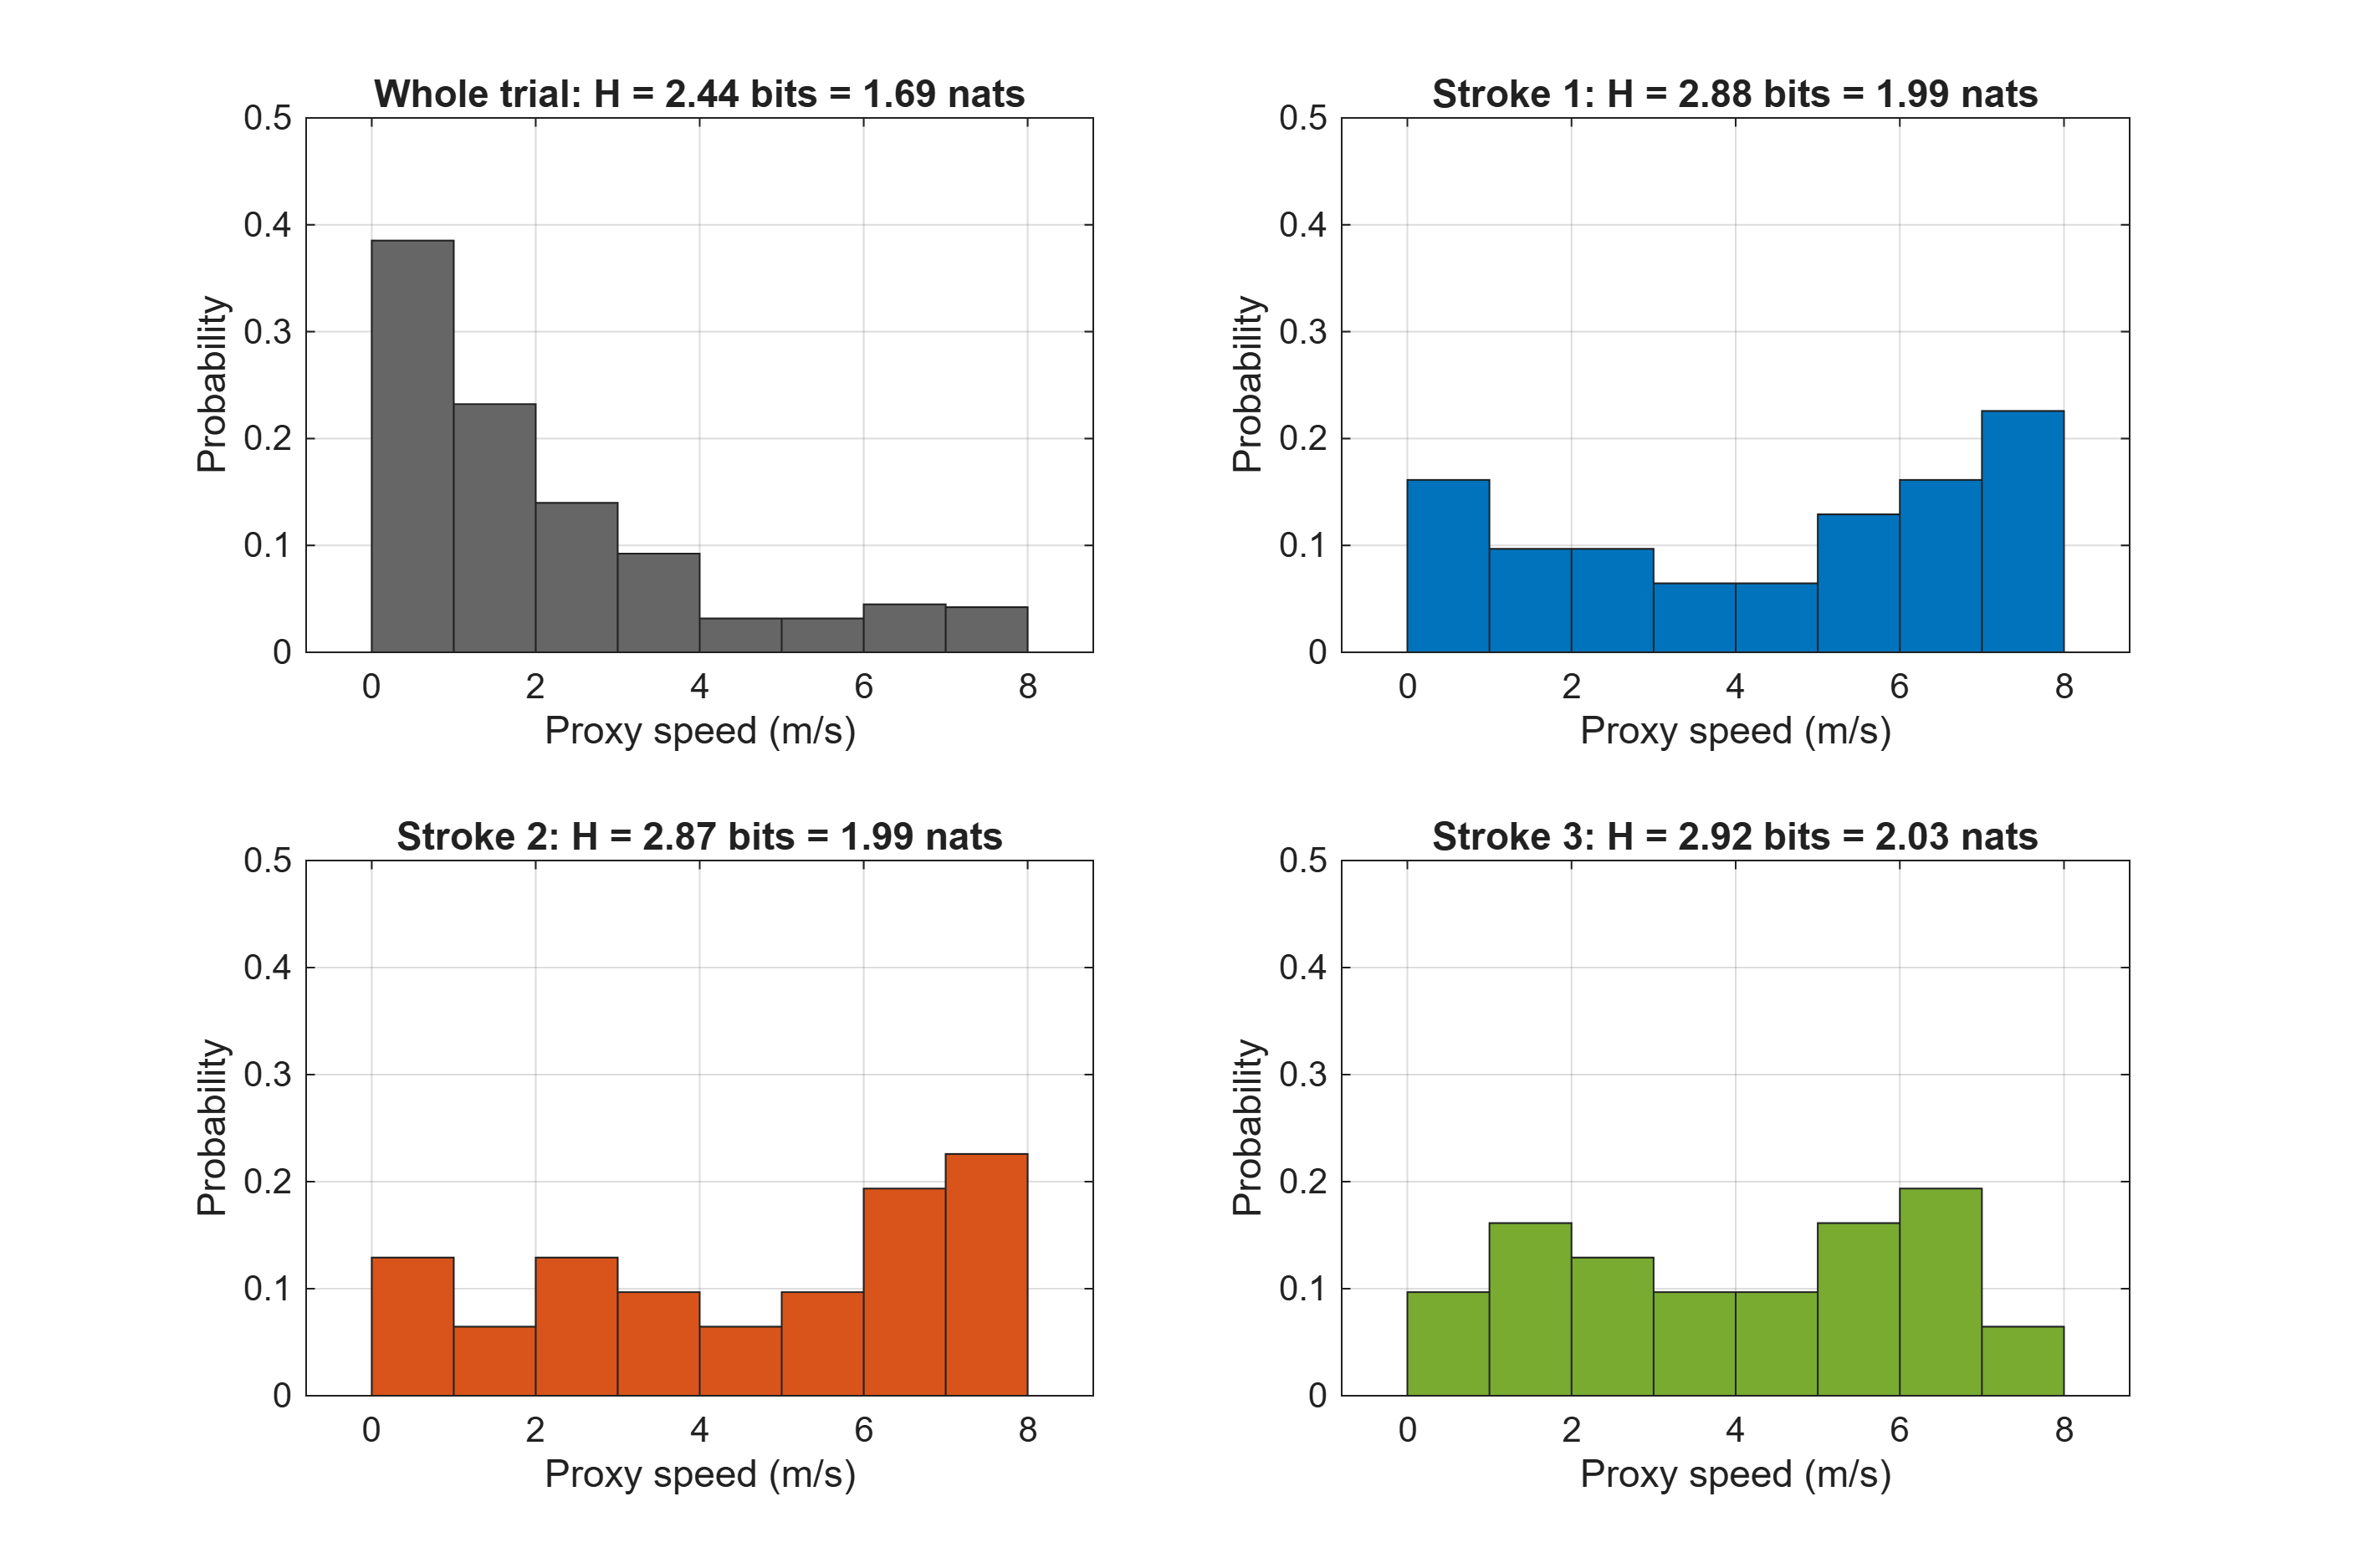
\includegraphics[width=0.7\linewidth]{Fig2_speed_histograms.png}\caption{Speed-occupancy distributions}\end{subfigure}
    \caption{(a) Proxy speed with the three stroke windows. (b) Speed-occupancy distributions with their entropies in bits and nats (see also \texttt{Fig7\_entropy\_bits\_nats.png}).}\label{fig:entropy}
\end{figure}

\subsection{Kullback--Leibler divergence between strokes}

The KL divergence $\KL(P\Vert Q)=\sum_i p_i\log_2(p_i/q_i)$ is the extra number of bits needed when data distributed as $P$ are coded with a code built for $Q$. It is \textbf{not symmetric} and is zero only if $P=Q$. A pseudo-count of 0.5 per bin (Jeffreys smoothing) avoids empty bins.

\begin{table}[ht]
    \centering
    \caption{$\KL(\text{row}\Vert\text{column})$ of the proxy-speed occupancy, in bits \tagobs. In nats multiply by 0.693.}\label{tab:kl}
    \footnotesize
    \begin{tabularx}{\textwidth}{@{}l c c c Y@{}}
        \toprule
        \textbf{P \textbackslash\ Q} & \textbf{S1} & \textbf{S2} & \textbf{S3} & \textbf{Reading}                                \\
        \midrule
        S1                           & 0           & 0.032       & 0.196       & S1 and S2 are almost the same speed profile     \\
        S2                           & 0.032       & 0           & 0.205       & S3 is the least similar stroke                  \\
        S3                           & 0.158       & 0.180       & 0           & Lower peak speed and a different height profile \\
        \bottomrule
    \end{tabularx}
\end{table}

\begin{figure}[ht]
    \centering
    \begin{subfigure}{0.48\textwidth}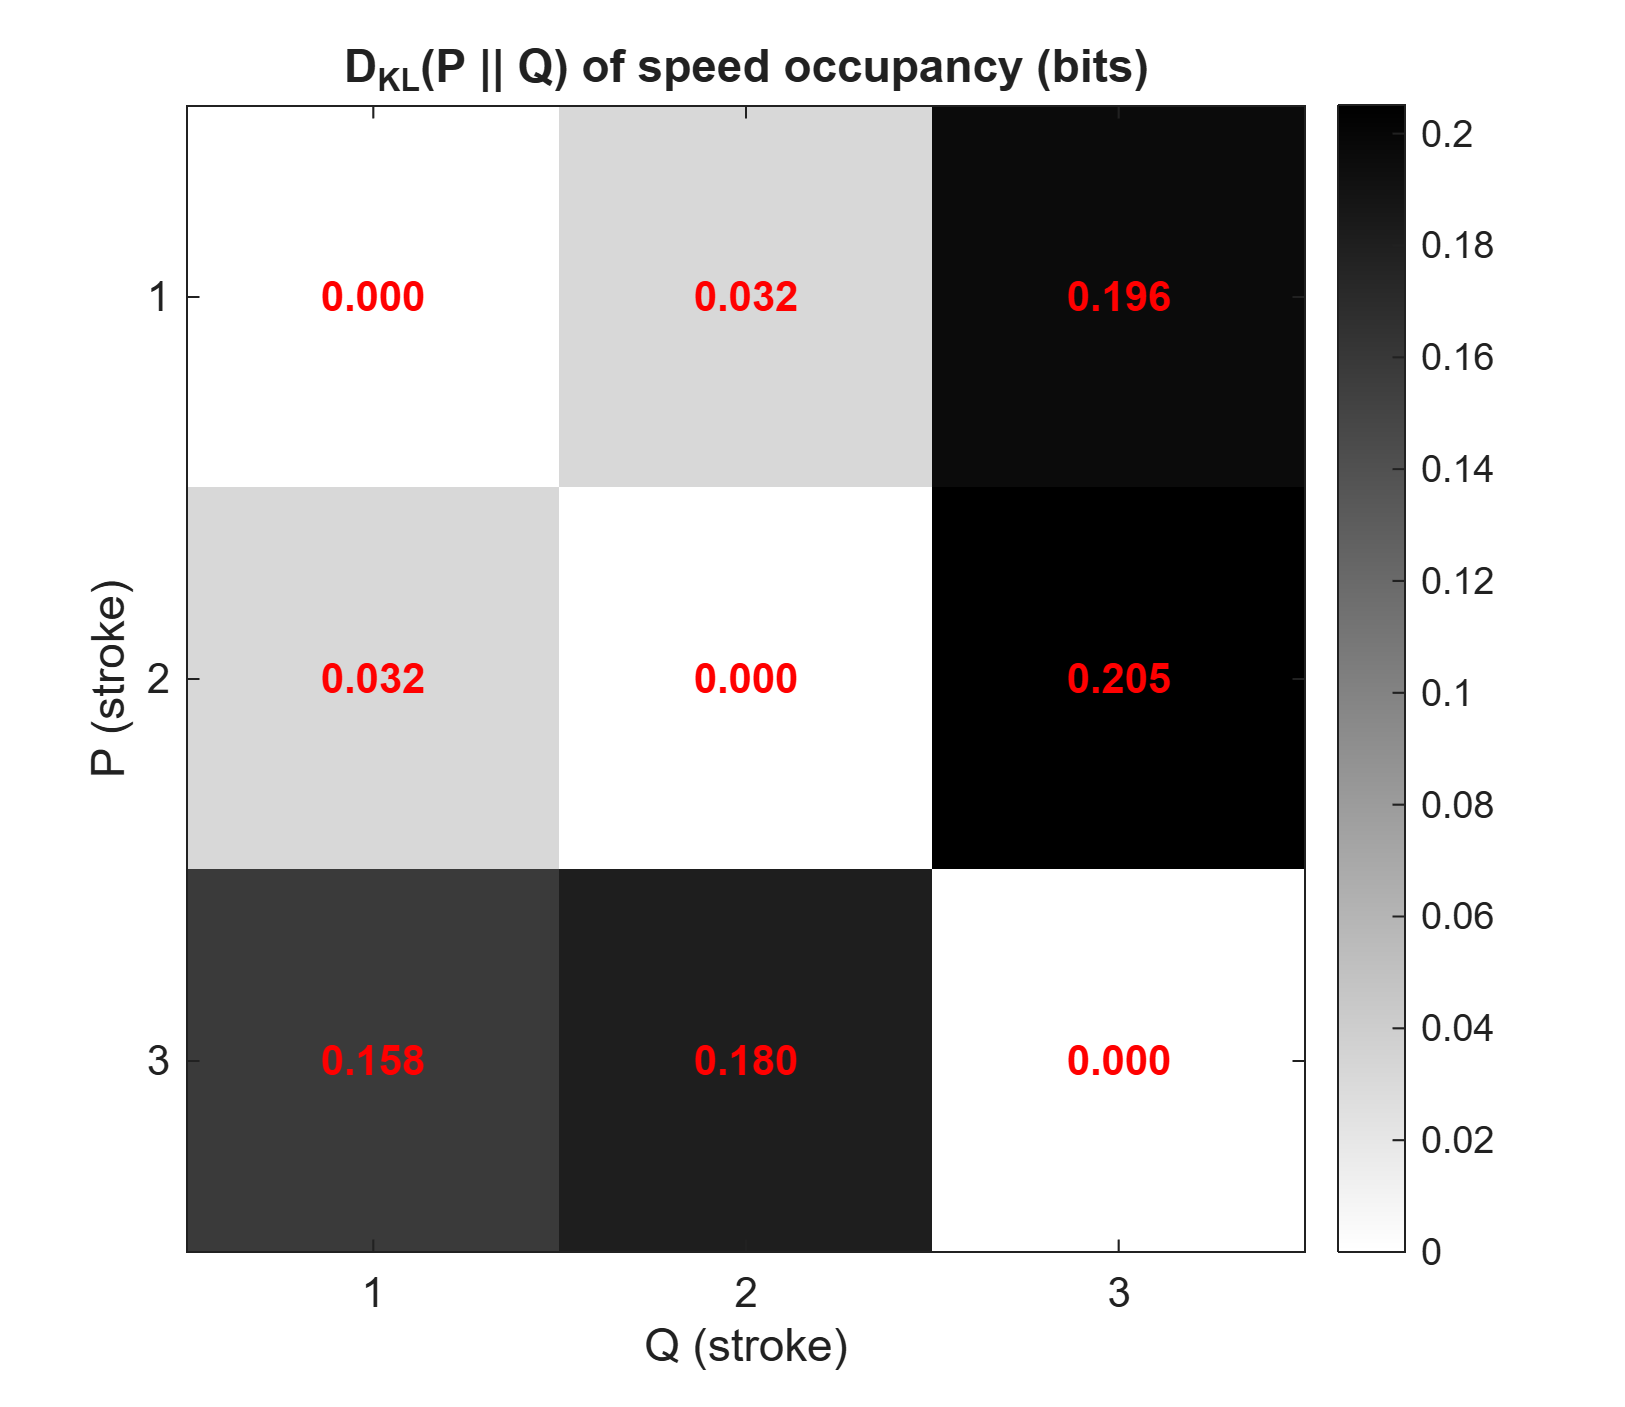
\includegraphics[width=\linewidth]{Fig5_KL_matrix.png}\caption{KL matrix between strokes}\end{subfigure}\hfill
    \begin{subfigure}{0.48\textwidth}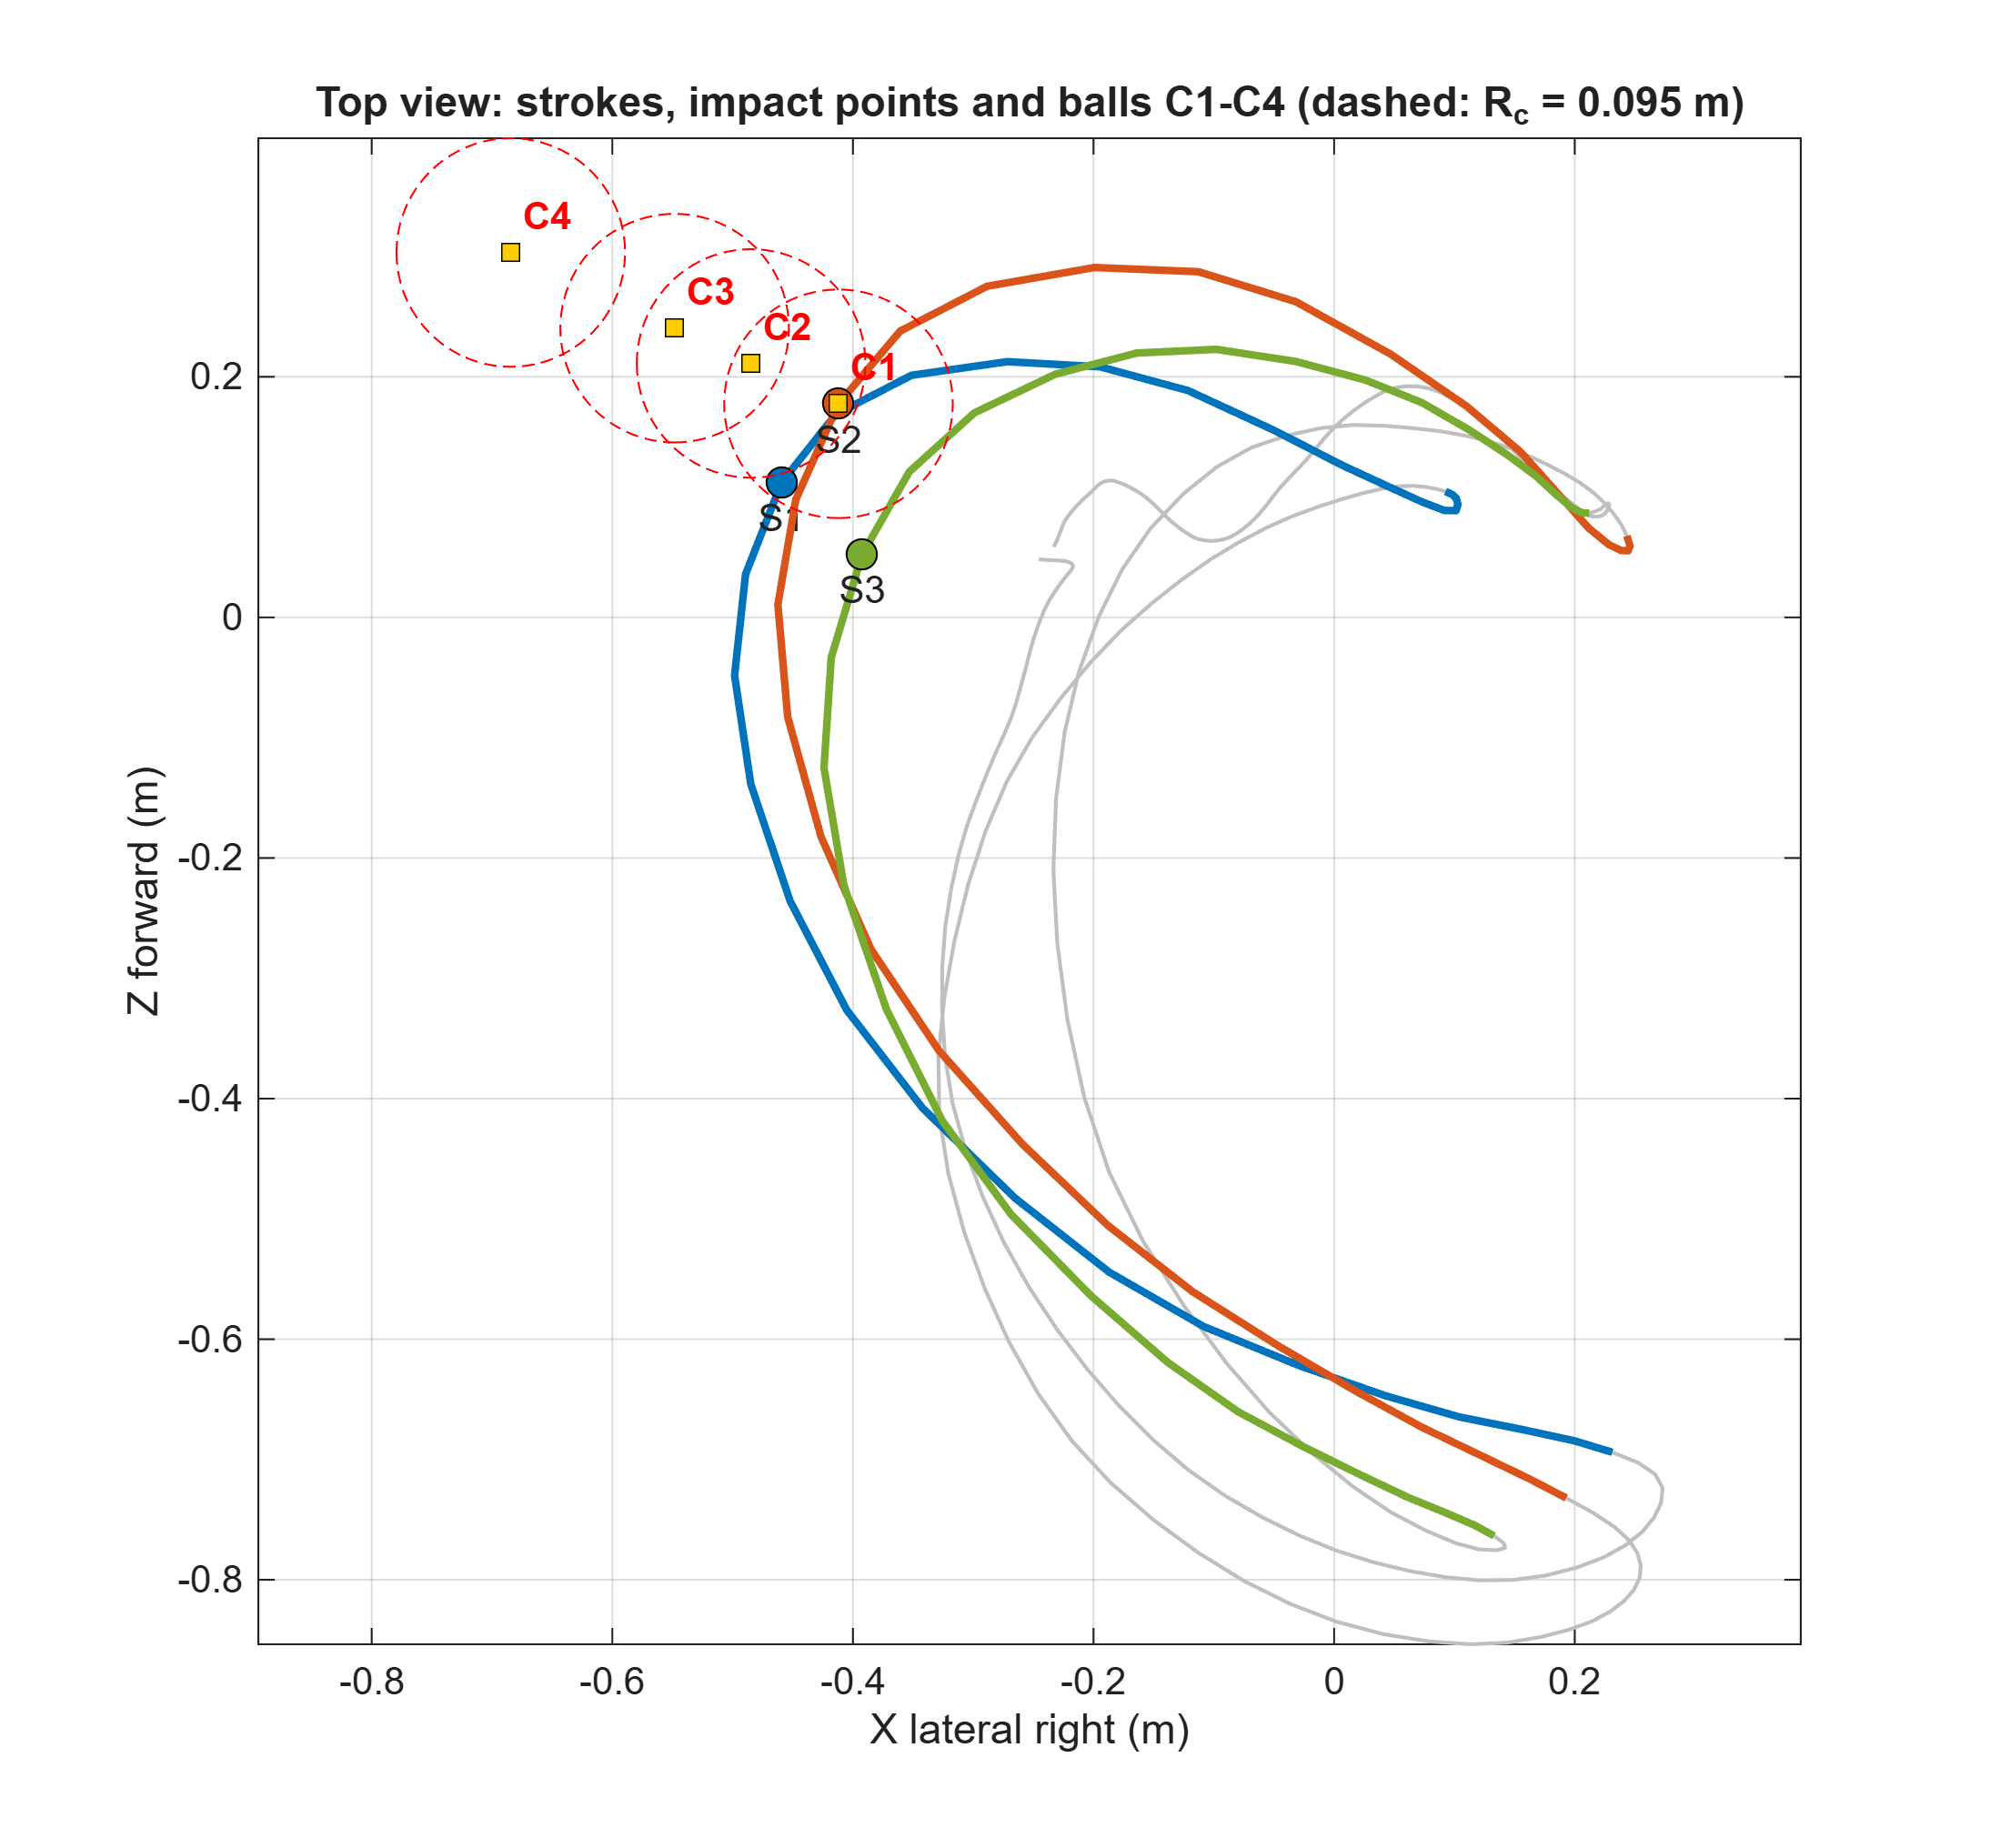
\includegraphics[width=\linewidth]{Fig3_topview_impacts.png}\caption{Top view of paths, impacts, balls C1--C4}\end{subfigure}
    \caption{(a) KL matrix between strokes. (b) Top view of the paths, impact points and the balls C1--C4 with their $\Rc$ circles.}\label{fig:kl}
\end{figure}

A second use of KL is \tagprop{} for the judgment data: $\KL(P_{\mathrm{obs}}\Vert P_{\mathrm{ideal}})$ between the observed proportion of ``possible'' responses per offset and the criterion (smoothed), computed per camera view; it measures, in bits, how far each viewpoint leaves the observer from the ideal.

\subsection{Conditional problems with two events}

Each problem uses a $2\times2$ table of two events and applies $P(B\given A)=P(A\cap B)/P(A)$ and Bayes' theorem $P(A\given B)=P(B\given A)P(A)/P(B)$. Mutual information $I(A;B)=\sum p(a,b)\log_2\frac{p(a,b)}{p(a)p(b)}$ measures how many bits one event tells about the other.

\paragraph{Problem 1 -- Frames: is a fast racket informative about contact?} $A$ = proxy speed $\ge\SI{4}{\meter\per\second}$ (57 of 379 frames); $B$ = proxy within $\Rc$ of the ball (contact frame). Counts over all frames:

\begin{table}[ht]
    \centering
    \caption{Frame counts for Problem 1 \tagsim.}\label{tab:p1}
    \footnotesize
    \begin{tabular}{@{}l c c c l@{}}
        \toprule
        \textbf{Counts (frames)}  & \textbf{$B$ contact} & \textbf{$B$ no contact} & \textbf{Total} & \textbf{Quantities}        \\
        \midrule
        C1 ($d=0.00$ m): $A$ fast & 3                    & 54                      & 57             & $P(B)=3/379=0.0079$        \\
        C1: $A$ slow              & 0                    & 322                     & 322            & $P(B\given A)=3/57=0.0526$ \\
        C2 ($d=0.08$ m): $A$ fast & 1                    & 56                      & 57             & $P(B)=1/379=0.0026$        \\
        C2: $A$ slow              & 0                    & 322                     & 322            & $P(B\given A)=1/57=0.0175$ \\
        \bottomrule
    \end{tabular}
\end{table}

\emph{Solution.} Bayes: $P(A\given B)=P(B\given A)P(A)/P(B)=0.0526\times0.1504/0.0079=\mathbf{1.00}$ (every contact frame is a fast frame); $P(B\given\text{slow})=0$. Mutual information $I(A;B)=\mathbf{0.022}$ bits (C1) and $\mathbf{0.007}$ bits (C2). Self-information (surprisal) of a contact frame: $-\log_2P(B)=\mathbf{6.98}$ bits (C1), $\mathbf{8.57}$ bits (C2). C3 and C4 have no contact frames, so $P(B)=0$ and $I=0$. \emph{Meaning:} contact is rare and short. At \SI{7.8}{\meter\per\second} the proxy moves \SI{0.13}{\meter} per frame, so a contact sphere of diameter \SI{0.19}{\meter} is crossed in about one or two frames ($\approx\SI{16.7}{\milli\second}$), which is why the timing demand is high.

\paragraph{Problem 2 -- Stroke trials: does near/far predict interception?} Using the three strokes against all four ball positions gives 12 stroke-trials. $A$ = ball near ($d\le\SI{0.08}{\meter}$) or far ($d\ge\SI{0.15}{\meter}$); $B$ = the stroke's closest approach is $\le\Rc$.

\begin{table}[ht]
    \centering
    \caption{Trial counts for Problem 2 \tagsim.}\label{tab:p2}
    \footnotesize
    \begin{tabular}{@{}l c c c l@{}}
        \toprule
        \textbf{Counts (trials)} & \textbf{$B$ intercept} & \textbf{$B$ no intercept} & \textbf{Total} & \textbf{Quantities}               \\
        \midrule
        $A$ near (C1, C2)        & 4                      & 2                         & 6              & $P(B\given\text{near})=4/6=0.667$ \\
        $A$ far (C3, C4)         & 0                      & 6                         & 6              & $P(B\given\text{far})=0$          \\
        Total                    & 4                      & 8                         & 12             & $P(B)=1/3$                        \\
        \bottomrule
    \end{tabular}
\end{table}

\emph{Solution.} Bayes: $P(\text{near}\given B)=0.667\times0.5/0.333=\mathbf{1.00}$. $H(B)=H(1/3)=0.918$ bits; $H(B\given A)=0.5\times0.918+0.5\times0=0.459$ bits; hence $I(A;B)=\mathbf{0.459}$ bits, half of the uncertainty about the outcome. Using the four conditions separately (C1: 3/3, C2: 1/3, C3: 0/3, C4: 0/3) the information is \textbf{0.689} bits of 0.918 bits.

\paragraph{Problem 3 -- Which stroke intercepts, and what is the probability?}

\begin{table}[ht]
    \centering
    \caption{Closest approach \dmin\ (m) per stroke window; $^{*}$ = intercept \tagsim. Linear interpolation between frames lowers \dmin\ by at most 0.008 m (e.g.\ C1, S1: 0.075 m) and changes no verdict.}\label{tab:p3}
    \footnotesize
    \begin{tabular}{@{}l c c c c l@{}}
        \toprule
        \textbf{Condition} & \textbf{S1} & \textbf{S2} & \textbf{S3} & \textbf{Intercepts $s/3$} & \textbf{Posterior mean of $P$(intercept)} \\
        \midrule
        C1, $d=0.00$ m     & $0.083^{*}$ & $0.000^{*}$ & $0.083^{*}$ & 3                         & 0.80, Beta(4,1)                           \\
        C2, $d=0.08$ m     & 0.104       & $0.080^{*}$ & 0.160       & 1                         & 0.40, Beta(2,3)                           \\
        C3, $d=0.15$ m     & 0.157       & 0.150       & 0.229       & 0                         & 0.20, Beta(1,4)                           \\
        C4, $d=0.30$ m     & 0.296       & 0.300       & 0.378       & 0                         & 0.20, Beta(1,4)                           \\
        \bottomrule
    \end{tabular}
\end{table}

\emph{Two events:} $A$ = ``stroke is S2 (the reference)'', $B$ = ``intercepts C2''. The $2\times2$ table (S2 and intercept: 1; S2 and no intercept: 0; other and intercept: 0; other and no intercept: 2) gives $P(B\given A)=1$, $P(B\given\neg A)=0$ and, by Bayes, $\mathbf{P(\text{S2}\given\text{intercept at C2})=1}$: the C2 verdict of the report holds only for the stroke on which the ball was placed. \emph{Bayes with a uniform prior:} after $s$ intercepts in $n=3$ strokes the posterior is Beta$(1+s,\,1+n-s)$; the 95\,\% credible interval is $[0.40,\,0.99]$ for C1, $[0.07,\,0.81]$ for C2 and $[0.006,\,0.60]$ for C3 and C4. The uncertainty about the next stroke is $H=0.72$, $0.97$, $0.72$ and $0.72$ bits for C1--C4: C2 is the most uncertain, as expected next to the boundary.

\begin{figure}[ht]
    \centering
    \begin{subfigure}{0.48\textwidth}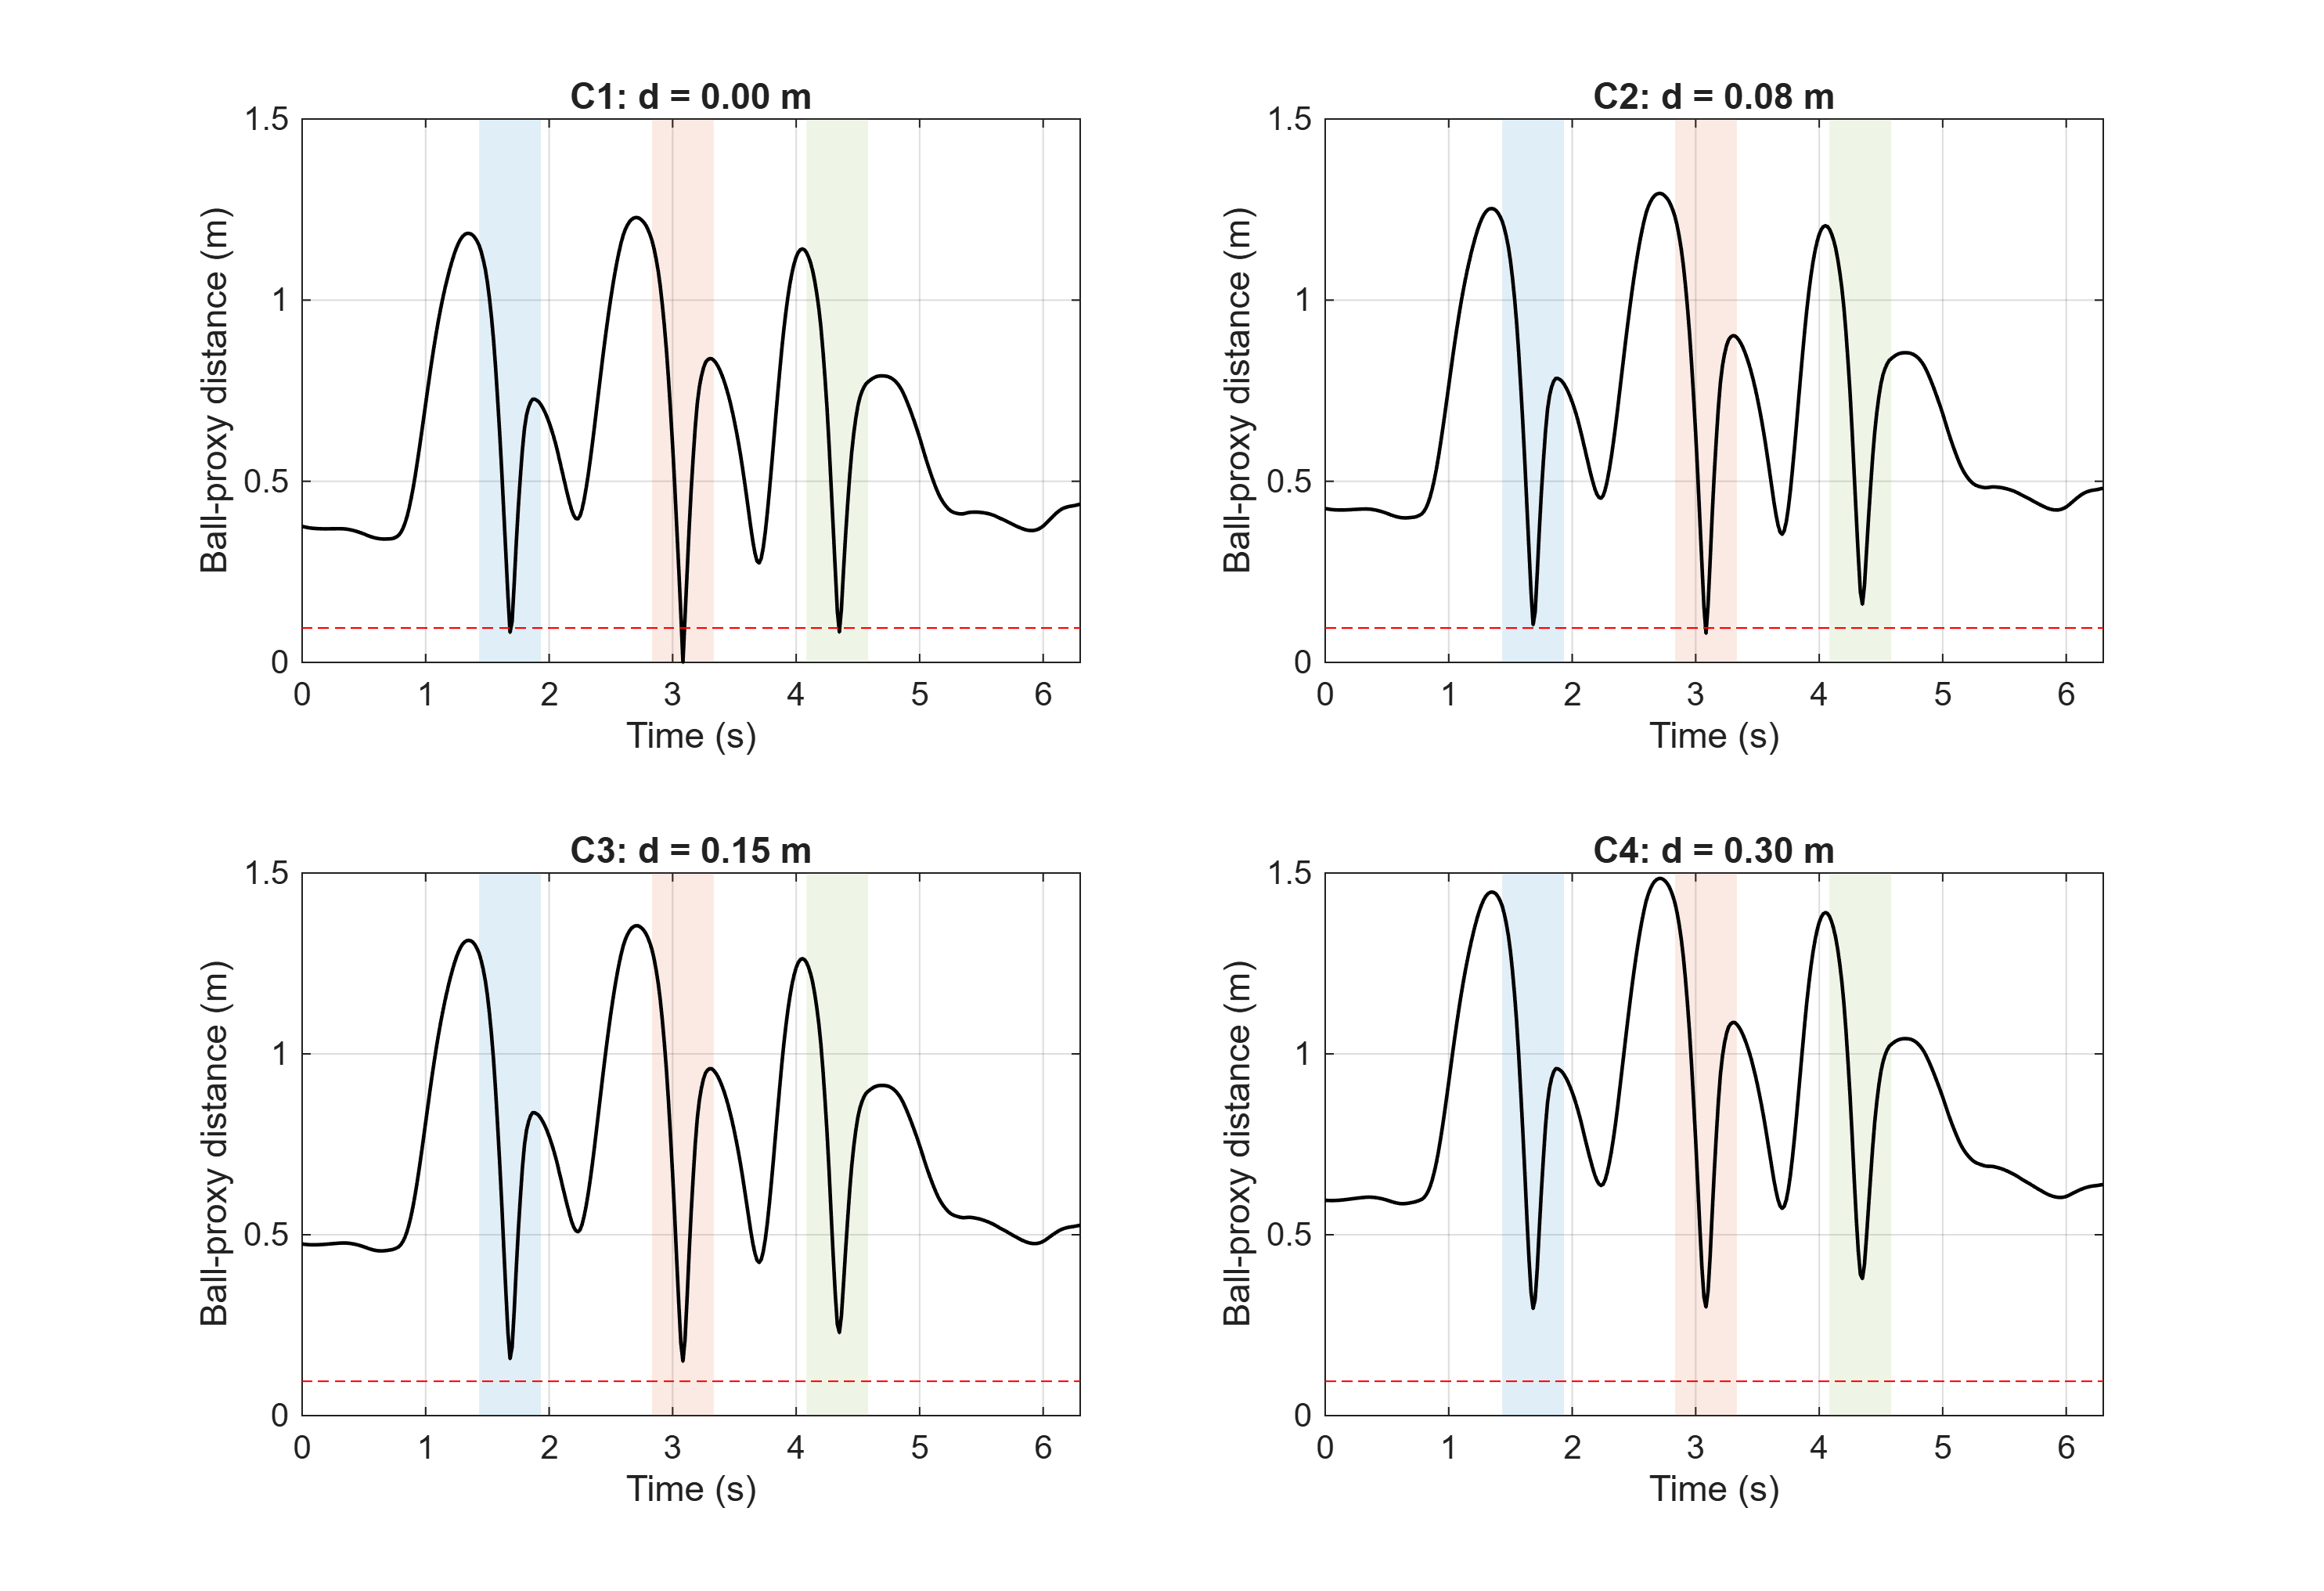
\includegraphics[width=\linewidth]{Fig4_distance_vs_time.png}\caption{Ball--proxy distance per condition}\end{subfigure}\hfill
    \begin{subfigure}{0.48\textwidth}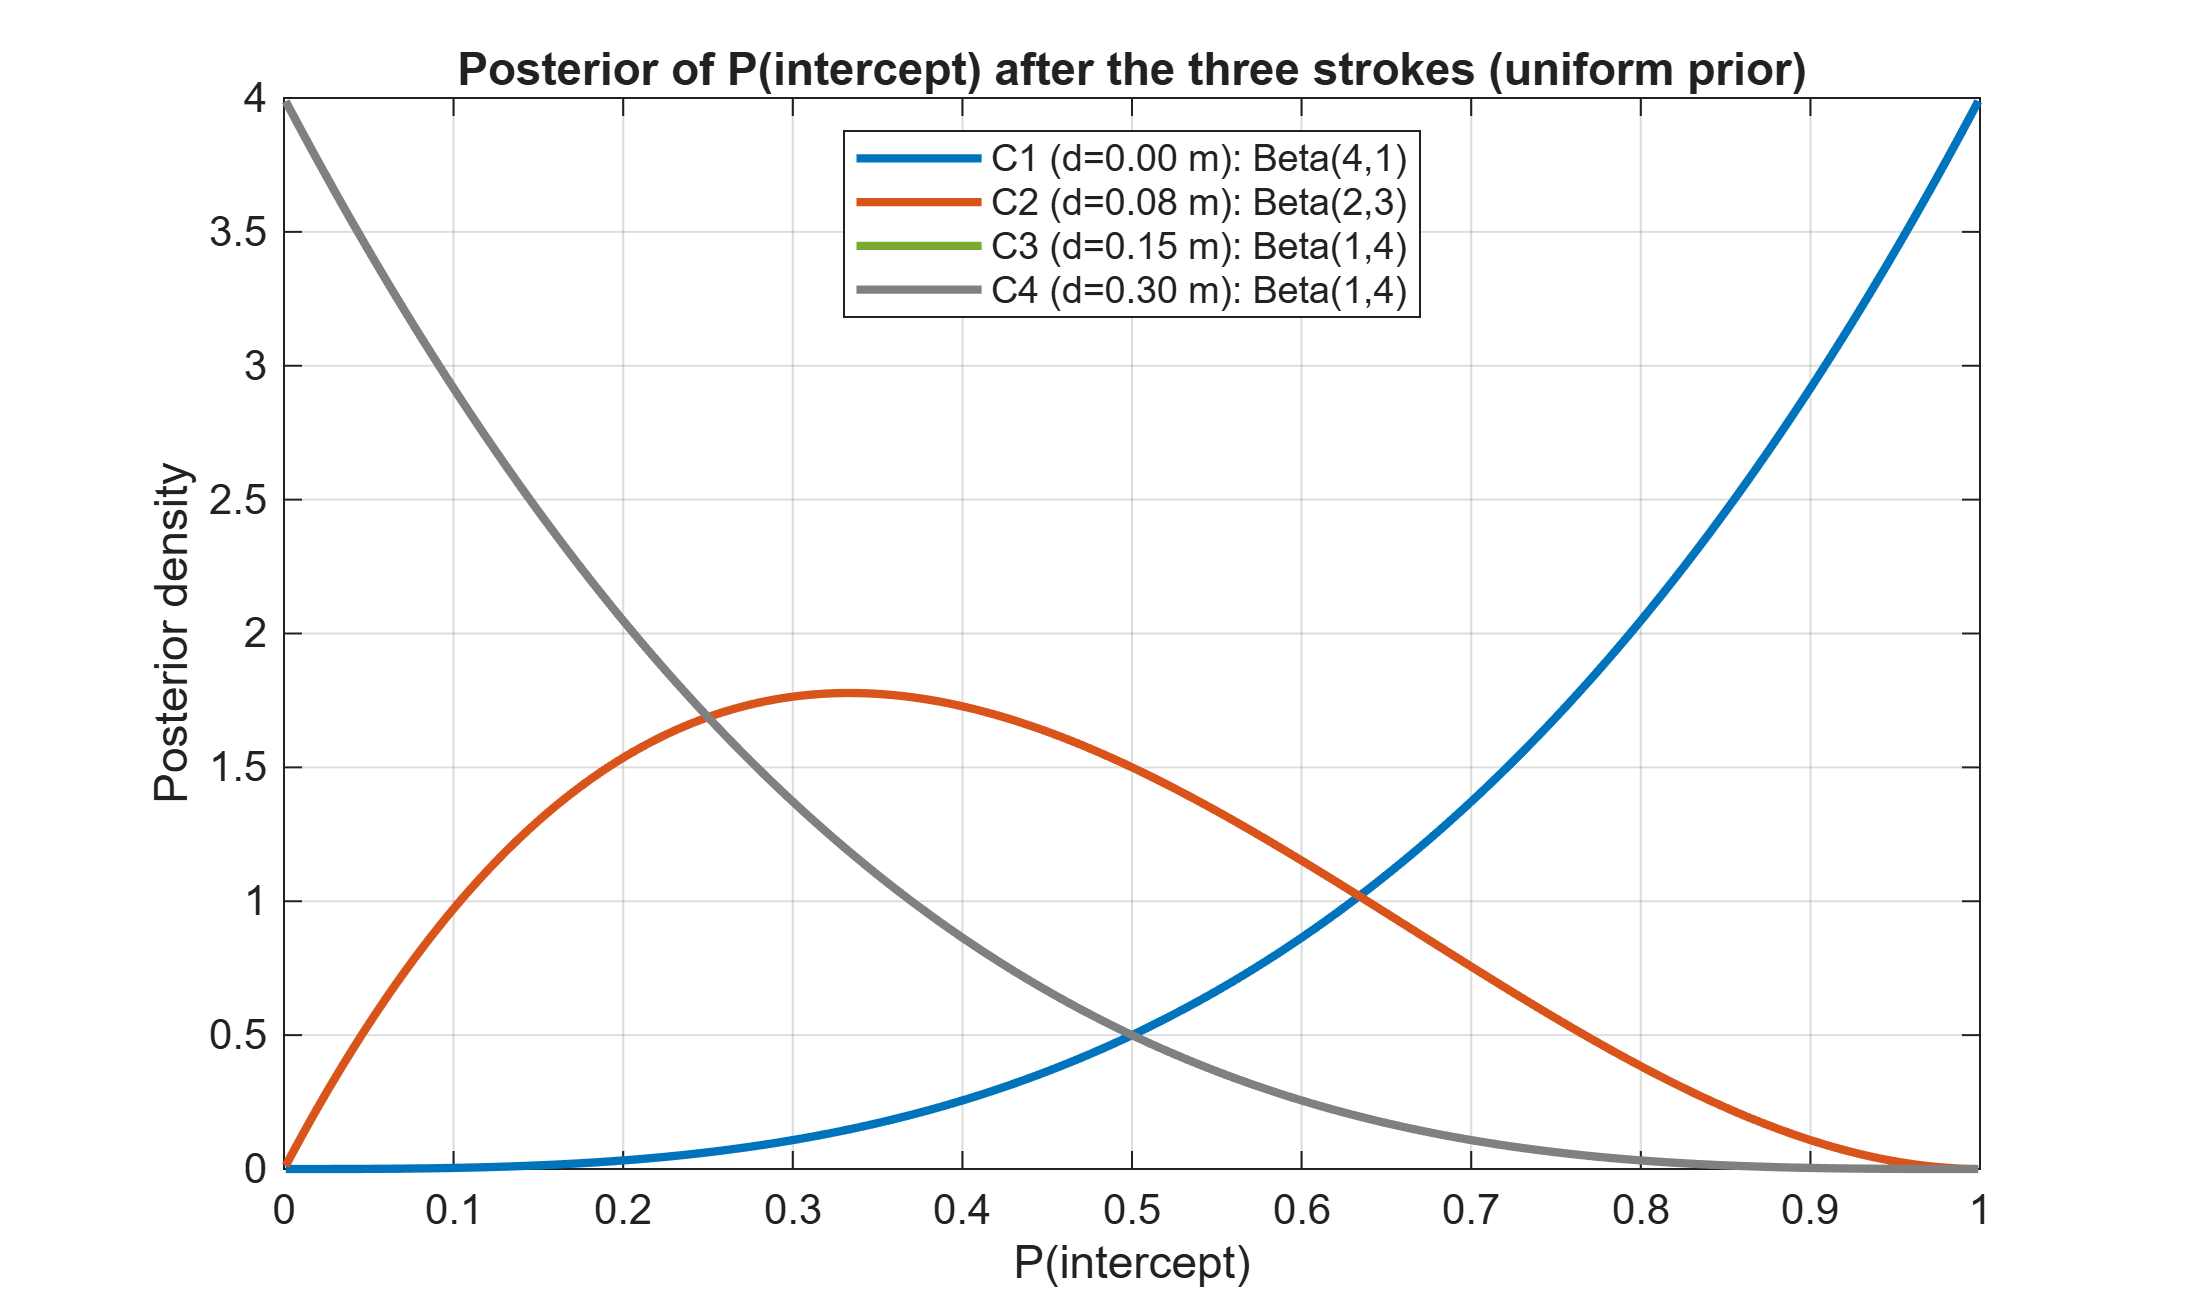
\includegraphics[width=\linewidth]{Fig6_beta_posteriors.png}\caption{Posterior of $P$(intercept)}\end{subfigure}
    \caption{(a) Ball--proxy distance per condition, with $\Rc$ and the three stroke windows. (b) Posterior distributions of $P$(intercept) per condition.}\label{fig:beta}
\end{figure}

\paragraph{Problem 4 -- How much do two extra strokes teach us? (KL as information gain)} With a uniform prior, the predictive probability of an intercept after $s$ of $n$ strokes is $(s+1)/(n+2)$. After the reference stroke only it is $q=(s_1+1)/3$; after all three it is $p=(s+1)/5$. The information gained is the KL divergence of the Bernoulli distributions:

\begin{table}[ht]
    \centering
    \caption{Information gained by two extra strokes.}\label{tab:p4}
    \footnotesize
    \begin{tabular}{@{}l c c c c@{}}
        \toprule
        \textbf{Condition} & $q$ (1 stroke) & $p$ (3 strokes) & $\KL(p\Vert q)$ bits & $\KL(p\Vert q)$ nats \\
        \midrule
        C1                 & 0.667          & 0.800           & 0.063                & 0.044                \\
        C2                 & 0.667          & 0.400           & 0.214                & 0.148                \\
        C3                 & 0.333          & 0.200           & 0.063                & 0.044                \\
        C4                 & 0.333          & 0.200           & 0.063                & 0.044                \\
        \bottomrule
    \end{tabular}
\end{table}

\emph{Meaning:} C2 gains the most (0.214 bits) because the extra strokes contradict the single-stroke verdict (intercept) the most.

\paragraph{Problem 5 -- Ideal observer and Bayes (\tagill{}, to be replaced by real judgments)} Let $F$ = ``ball feasible'' (C1, C2; prior 0.5) and $J$ = ``observer says possible''. Assume hit rate $P(J\given F)=0.85$ and false-alarm rate $P(J\given\neg F)=0.20$ (\textbf{assumed values, not data}).

\begin{table}[h]
    \centering
    \caption{Joint probabilities for Problem 5 \tagill.}\label{tab:p5}
    \footnotesize
    \begin{tabular}{@{}l c c c@{}}
        \toprule
        \textbf{Joint probability} & \textbf{$J$ yes} & \textbf{$J$ no} & \textbf{Total} \\
        \midrule
        $F$ feasible               & 0.425            & 0.075           & 0.500          \\
        not $F$                    & 0.100            & 0.400           & 0.500          \\
        Total                      & 0.525            & 0.475           & 1.000          \\
        \bottomrule
    \end{tabular}
\end{table}

\emph{Solution.} Bayes: $P(F\given\text{yes})=0.85\times0.5/0.525=\mathbf{0.810}$; $P(F\given\text{no})=0.15\times0.5/0.475=\mathbf{0.158}$. $I(F;J)=\mathbf{0.332}$ bits of the 1 bit available ($H(F)=1$ bit); $d'=z(0.85)-z(0.20)=\mathbf{1.88}$. With the real judgments, build one such table \textbf{per camera view} (Section~\ref{sec:judgment-curves}): the view with the largest $I(F;J)$ is the one whose optical information specifies the affordance best, and the occlusion in the behind view (H2) predicts the smallest value.

\subsection{Interpretation and limits}

\begin{itemize}
    \item \textbf{Affordance as graded information:} the three strokes show that the geometric boundary is blurred by about \SI{7}{\centi\meter} of stroke-to-stroke variability; C1 is feasible in 3/3 strokes, C2 in 1/3, C3 and C4 in 0/3.
    \item \textbf{Bits quantify what each event tells us:} knowing near/far removes 0.46 bits of the 0.92 bits of uncertainty about interception; a perfect observer could transmit at most $H(F)=1$ bit per judgment.
    \item \textbf{Limits:} $n=3$ strokes; frames are autocorrelated; entropies depend on the bin width (\SI{1}{\meter\per\second}) and are biased low for 31 frames; KL uses a 0.5 pseudo-count; Problem~5 uses assumed rates; the criterion is evaluated on \SI{60}{\hertz} samples ($\approx\SI{0.13}{\meter}$ per frame at peak speed), although interpolation changes no verdict.
\end{itemize}